\section{Privately Programmable Pseudorandom Set with List Decoding}
\label{sec:ppps}
\subsection{Definition}
\label{sec:ppps-defn}
\paragraph{Distribution of set $\mcal{D}_n$.}
We want to construct a pseudorandom set 
whose distribution
emulates a set $S \subset \{0, 1, \ldots, n-1\}$ of size $\sqrt{n}$ 
sampled from the following distribution
denoted $\mcal{D}_n$ --- 
we assume that $n$ is a perfect forth ($n^{1/4}$ is an integer): 
\begin{itemize}[leftmargin=5mm,itemsep=1pt]
\item 
Divide the $n$ elements into $\sqrt{n}$ chunks indexed
with $0, 1, \ldots, \sqrt{n}-1$, 
where chunk $i$ contains the elements  
$[\chunkid \cdot \sqrt{n}, \ (\chunkid+1) \cdot \sqrt{n} - 1]$
\item 
For each chunk $\chunkid \in \{0, 1, \ldots, \sqrt{n}-1\}$, 
sample a random offset $\delta_\chunkid \getr \{0, 1, \ldots, \sqrt{n}-1\}$.
\item 
Output the following set $S := 
\{\chunkid \cdot \sqrt{n} + \delta_\chunkid \}_{\chunkid \in \{0, 1, \ldots, \sqrt{n}-1\}}$.
\end{itemize}

\paragraph{Offset representation of a set.}
For convenience, in the rest of the section,
we will always use an offset representation of a set, i.e.,
we will represent a set 
as 
$$S := \{\delta_0, \ldots, \delta_{\sqrt{n}-1}\}$$
where each $\delta_i \in \{0, \ldots, \sqrt{n}-1\}$
represents the relative
offset of the $i$-th element 
inside the $i$-th chunk.

\paragraph{Privately programmable pseudorandom set with list decoding.}
We introduce a new abstraction called a privately programmable pseudorandom set with list decoding that we utilize in our PIR constructions that follow. Intuitively, this primitive provides an algorithm to generate a secret key that represents pseudorandom subset of $\{0,\ldots,n-1\}$ with a specific distribution. Further, the primitive allows, given a key for a pseudorandom set, to produce a key for pseudorandom set that is the same as the starting set except for being programmed at a particular location with a specified value -- with the guarantee that the new key does not reveal the programmed location. Moreover, this primitive has a list decoding algorithm, that given a programmed key outputs a list of sets such that one of them is the one is the correct set that the key represents.


Formally, define a privately programmable pseudorandom set (\ppps) 
with list decoding
which emulates the distribution $\mcal{D}_n$:

\begin{itemize}[leftmargin=5mm,itemsep=1pt]
\item 
 $\sk \leftarrow {\sf Gen}(1^\lambda, n)$:
takes in the security parameter $1^\lambda$, the size
of the set $n$, and outputs a secret key $\sk$.
\item 
$S \leftarrow {\sf Set}(\sk)$:
takes in a secret key $\sk$, and expands it to a random set $S$
of size $\sqrt{n}$.
We sometimes write ${\sf Set}(\sk)[i]$ to denote the element in the $i$-th chunk for this set.
\item 
 $\sk', i \leftarrow {\sf Program}(\sk, \chunkid, \delta_\chunkid)$:
takes in a secret key $\sk$, a chunk identifier
$\chunkid \in \{0, 1, \ldots, \sqrt{n}-1\}$, 
a desired offset 
$\delta_\chunkid$
within the specified chunk 
$\chunkid$, 
 and 
outputs a programmed
key $\sk'$, and some auxiliary information 
$i$ that 
indicates which of the decoded set 
will be correct. 
\item 
 $\{S_0, \ldots, S_{L-1}\} \leftarrow {\sf ListDecode}(\sk')$:
takes in a programmed key $\sk'$ and 
outputs a list of sets $S_0, S_2, \ldots, S_{L-1}$, such that
one of them is the correctly programmed set corresponding to the key $\sk'$. 
\end{itemize}


\paragraph{Correctness.}
Correctness requires that 
for any $\lambda, n \in \mathbb{N}$, 
for any $\chunkid, \delta_\chunkid \in \{0, 1, \ldots, \sqrt{n}-1\}$, 
the following holds with probability 1:
%\begin{itemize}[leftmargin=5mm,itemsep=1pt]
%\item 
%$\sk \leftarrow {\sf Gen}(1^\lambda, n)$, 
%then $S := {\sf Set}(\sk)$ 
%is of size $\sqrt{n}$, and moreover,
%for each $\chunkid \in \{0, \ldots, \sqrt{n}-1\}, 
%$S[\chunkid]$ is an element belonging to the $\chunkid$-th chunk.
%\item 
let 
$\sk \leftarrow {\sf Gen}(1^\lambda, n)$, 
$\sk', i \leftarrow {\sf Program}(\sk, \chunkid, \delta_\chunkid)$, 
$S_0, \ldots, S_{L-1}
\leftarrow {\sf ListDecode}(\sk')$, 
it must be that 
$S_i$ is equal to the ${\sf Set}(\sk)$ 
but replacing 
the $\chunkid$-th element with 
$\delta_\chunkid$ instead.
%\end{itemize}

%\elaine{TODO: fill in}
\paragraph{Pseudorandomness.}
We say that a %privately programmable pseudorandom set scheme
\ppps scheme 
emulates  
$\mcal{D}_n$ iff 
the following two distributions are computationally indistinguishable:
\begin{itemize}[leftmargin=5mm,itemsep=1pt]
\item 
Sample $S \getr \mcal{D}_n$ and output $S$;
\item 
Sample $\sk \leftarrow {\sf Gen}(1^\lambda, n)$, output  
${\sf Set}(\sk)$.
\end{itemize}


\paragraph{Private programmability.}
We require that 
there exists a probabilistic polynomial time simulator ${\sf Sim}$ 
such that 
for any $n \in \mathbb{N}$ that is a perfect square
and polynomially bounded in $\lambda$, 
any $\chunkid \in \{0, 1, \ldots, \sqrt{n}-1\}$, 
any index $x$ that belongs to the $\chunkid$-th chunk,  
the outputs of the following experiments be computationally
indistinguishable:
\begin{itemize}[leftmargin=5mm,itemsep=1pt]
\item 
${\sf Real}$.
Sample $\sk \leftarrow {\sf Gen}(1^\lambda, n)$ subject to 
$x \in {\sf Set}(\sk)$, 
let $\delta_\chunkid \getr \{0, 1, \ldots, \sqrt{n}-1\}$,  
and let $\sk', \_ \leftarrow {\sf Program}(\sk, \chunkid, \delta_\chunkid)$, output $\sk'$.
\item 
${\sf Ideal}$.
Output ${\sf Sim}(1^\lambda, n)$.
%Sample $\sk \leftarrow {\sf Gen}(1^\lambda, n)$ and output $\sk$.
\end{itemize}

\paragraph{Efficiency.}
In our PIR scheme later, we need a programmed key $\sk'$ to
have size at most $O_\lambda(n^{1/4})$.
Further, 
the size of the decoded list
$L = n^{1/4}$.
Na\"ively, since each set has size $\sqrt{n}$, it would
take $n^{3/4}$ space to represent
the $L$ decoded sets. 
However, we want our scheme to satisfy a non-trivial notion
of efficiency, that is, 
it takes only $O(\sqrt{n})$
space to represent all $L$ decoded sets. 
Specifically, the compression is possible
because the $L$ decoded sets are correlated.



\subsection{Construction}
\label{sec:ppps-constr}
%Let 
%$\PRF: \{0, 1\}^\lambda \times \{0, 1\}^{\frac{1}{2}\log n} \rightarrow 
%\{0, 1\}^{\frac{1}{2}\log n}
%$denote a pseudorandom function.
\paragraph{Intuition.}
In our construction, we will divide the $\sqrt{n}$ {\it chunks}
into $n^{1/4}$ {\it superblocks}
where the $i$-th superblock contains 
the $i$-th group of $n^{1/4}$
consecutive chunks.

To program a \ppps key in some chunk $\ell$ with the specified
offset $\widetilde{\delta}$, 
we first expand the \ppps key to $n^{1/4}$ superblock keys
denoted $k_0, \ldots, k_{n^{1/4}-1}$.
Let $i$ be the superblock corresponding 
to chunk $\ell$. We then replace
$k_{i}$ with a randomly sampled superblock key $\widetilde{k}_{i}$.
We than expand $k_i$ into $n^{1/4}$
offsets denoted $\delta_0, \ldots, \delta_{n^{1/4}-1}$, 
one corresponding to each chunk contained in the $i$-th superblock.
Suppose chunk $\ell$ corresponds to the $j$-th chunk within the $i$-th
superblock. 
We then replace $\delta_j$ 
with the desired $\tilde{\delta}$. 
The programmed key is the combination of  
$k_0, \ldots, k_{i-1}, \widetilde{k}_{i}, k_{i+1}, \ldots, k_{n^{1/4}-1}$,
and 
$\delta_0, \ldots, \delta_{j-1}, \widetilde{\delta}, \delta_{j+1}, 
\ldots, \delta_{n^{1/4}-1}$.
Given this programmed key, we do not know 
which 
superblock should contain the expanded offsets 
$\delta_0, \ldots, \delta_{j-1}, \widetilde{\delta}, \delta_{j+1}, 
\ldots, \delta_{n^{1/4}-1}$.
However, we can generate
a list of $n^{1/4}$ candidate sets 
by plugging in the offsets 
$\delta_0, \ldots, \delta_{j-1}, \widetilde{\delta}, \delta_{j+1}, 
\ldots, \delta_{n^{1/4}-1}$ into 
each of the $n^{1/4}$ superblocks.
One of them must be the true programmed set. 

%and we replace the superblock key where $\ell$ resides 
%with a random superblock key.





\paragraph{Detailed \ppps construction.}
Henceforth, 
let 
$\PRF_1: \bits^{\lambda}\times \bits^{\frac{\log n}{4}}\to
\bits^{\lambda}$, and 
$\PRF_2:\bits^{\lambda}\times \bits^{\frac{\log n}{4}}\to
\bits^{\frac{\log n}{2}}$
be two pseudorandom functions.

\begin{itemize}[leftmargin=5mm,itemsep=1pt]
\item 
 ${\sf Gen}(1^\lambda, n)$: Sample a $\PRF_1$ key $\sk$ and output $\sk$.
\item 
${\sf Set}(\sk)$:
\begin{enumerate}[leftmargin=5mm,itemsep=1pt]
\item 
First, expand $\sk$ to $n^{1/4}$ superblock keys:
\begin{equation}
\forall i \in \{0, \ldots, n^{1/4}-1\}: \ k_i = \PRF_1(\sk, i)
\label{eqn:expandsb}
\end{equation}
\item 
Next, for each superblock $i \in \{0, \ldots, n^{1/4}-1\}$, compute
the pseudorandom offset 
for each of its $n^{1/4}$ chunks, that is:
\begin{equation}
\forall i, j  \in \{0, \ldots, n^{1/4}-1\}: \ 
%\delta_{i \cdot n^{1/4} + j} = \PRF(k_i, j)
\delta_{i, j} = \PRF_2(k_i, j)
\label{eqn:expandchunk}
\end{equation}
\item 
Define the alias $\delta_{i \cdot n^{1/4} + j} := \delta_{i, j}$, 
and output 
$S := \{\delta_\chunkid\}_{\chunkid \in \{0, \ldots, \sqrt{n}-1\}}$.
\end{enumerate}
\item 
 ${\sf Program}(\sk, \chunkid, \widetilde{\delta})$:
\begin{enumerate}[leftmargin=5mm,itemsep=1pt]
\item 
Expand $\sk$ to $n^{1/4}$
superblock keys denoted $k_0, \ldots, k_{n^{1/4} -1}$ as in
\Cref{eqn:expandsb}.
\item 
Let $i := \lfloor\chunkid/n^{1/4}\rfloor$ 
be the superblock containing the $\chunkid$-th chunk,
let $j := \chunkid \mod n^{1/4}$ be the index of chunk $\chunkid$ within 
superblock $i$. 
\item 
Sample a fresh PRF key $\widetilde{k}_i$ to replace $k_i$ with. 
\item  
For $j' \in \{0, 1, \ldots, n^{1/4} -1\}$, compute 
$\delta_{j'} = \PRF_2(k_i, j')$.

\item 
Output the following:
\[
\sk' := 
\left(
\begin{array}{ll}
(k_0, \ldots, k_{i-1}, \widetilde{k}_i, k_{i+1}, \ldots, k_{n^{1/4}-1}),\\[1pt]
(\delta_0, \ldots, \delta_{j-1}, \widetilde{\delta}, \delta_{j+1}, 
\ldots, \delta_{n^{1/4}-1}),\\[1pt]
\end{array}
\right), \quad i 
\]
\end{enumerate}

\item 
 ${\sf ListDecode}(\sk')$:
\begin{enumerate}[leftmargin=5mm,itemsep=1pt]
\item 
Parse $\sk' = (\{k_i\}_{i\in \{0, \ldots, n^{1/4}-1\}}, 
\{\delta^*_j\}_{j\in \{0, \ldots, n^{1/4}-1\}})$.
\item 
$\forall i, j  \in \{0, \ldots, n^{1/4}-1\}$, 
%compute $\delta_{i \cdot n^{1/4} + j}$
compute $\delta_{i, j}$
like in \Cref{eqn:expandchunk}, let 
$S$ be the matrix $S := \{\delta_{i, j}\}_{i, j 
\in \{0,1, \ldots, n^{1/4}-1\}}$.
%$S = \{\delta_0, \ldots, \delta_{n^{1/2} - 1}\}$.
\item 
For $i \in \{0, \ldots, n^{1/4}-1\}$, 
let $S_i$ be the same as
$S$ except for substituting the $i$-th row 
%$\{\delta_{i \cdot n^{1/4}}, \ldots, \delta_{(i+1) \cdot n^{1/4} - 1}\}$
with  
$\{\delta^*_j\}_{j\in \{0, \ldots, n^{1/4}-1\}}$.
In other words, 
\[
S_i := \left(
\begin{array}{lcr}
\delta_{0, 0}, &  \ldots, & \delta_{0, n^{1/4}-1}, \\
%\delta_{1, 0}, & \ldots, &\delta_{1,  n^{1/4}-1}, \\
%& \ldots, & \\ 
\ldots, & \ldots, & \ldots, \\ 
\delta_{i-1, 0}, & \ldots, &\delta_{i-1,  n^{1/4}-1}, \\
\delta^*_0, &\ldots, &\delta^*_{n^{1/4-1}}, \\
\delta_{i+1, 0}, & \ldots, &\delta_{i+1,  n^{1/4}-1}, \\
\ldots, & \ldots, & \ldots, \\ 
\delta_{n^{1/4} -1, 0}, &  \ldots, &\delta_{n^{1/4}-1, n^{1/4}-1}, 
%\delta_{(i+1)\cdot n^{1/4}}, \ldots
%\delta_{n^{1/2} -1}, 
\end{array}
\right)
\]
\item 
\ignore{
For $i \in \{0, \ldots, n^{1/4}-1\}$,
let $S_i := {\sf Flatten}(S'_i) + 
(0, 1, \ldots, \sqrt{n}-1) \cdot \sqrt{n}$.
where ${\sf Flatten}$ outputs
the vector obtained from concatenating all rows of the matrix,
and 
the $(0, 1, \ldots, \sqrt{n}-1) \cdot \sqrt{n}$
part converts the  
relative 
offsets to a list of indices from $\{0, \ldots, n-1\}$.
}
Output $({\sf Flatten}(S_0), \ldots, {\sf Flatten}(S_{n^{1/4}-1}))$
where ${\sf Flatten}$ outputs
the vector obtained from concatenating all rows of the matrix,


\ignore{
$({\sf Flatten}(S_0) + 
(0, 1, \ldots, \sqrt{n}-1) \cdot \sqrt{n}, 
\ldots, 
{\sf Flatten}(S_{n^{1/4} -1}) + 
(0, 1, \ldots, \sqrt{n}-1) \cdot \sqrt{n}, 
)$} 
\end{enumerate}
\end{itemize}

\begin{figure*}[t]
    \centering
    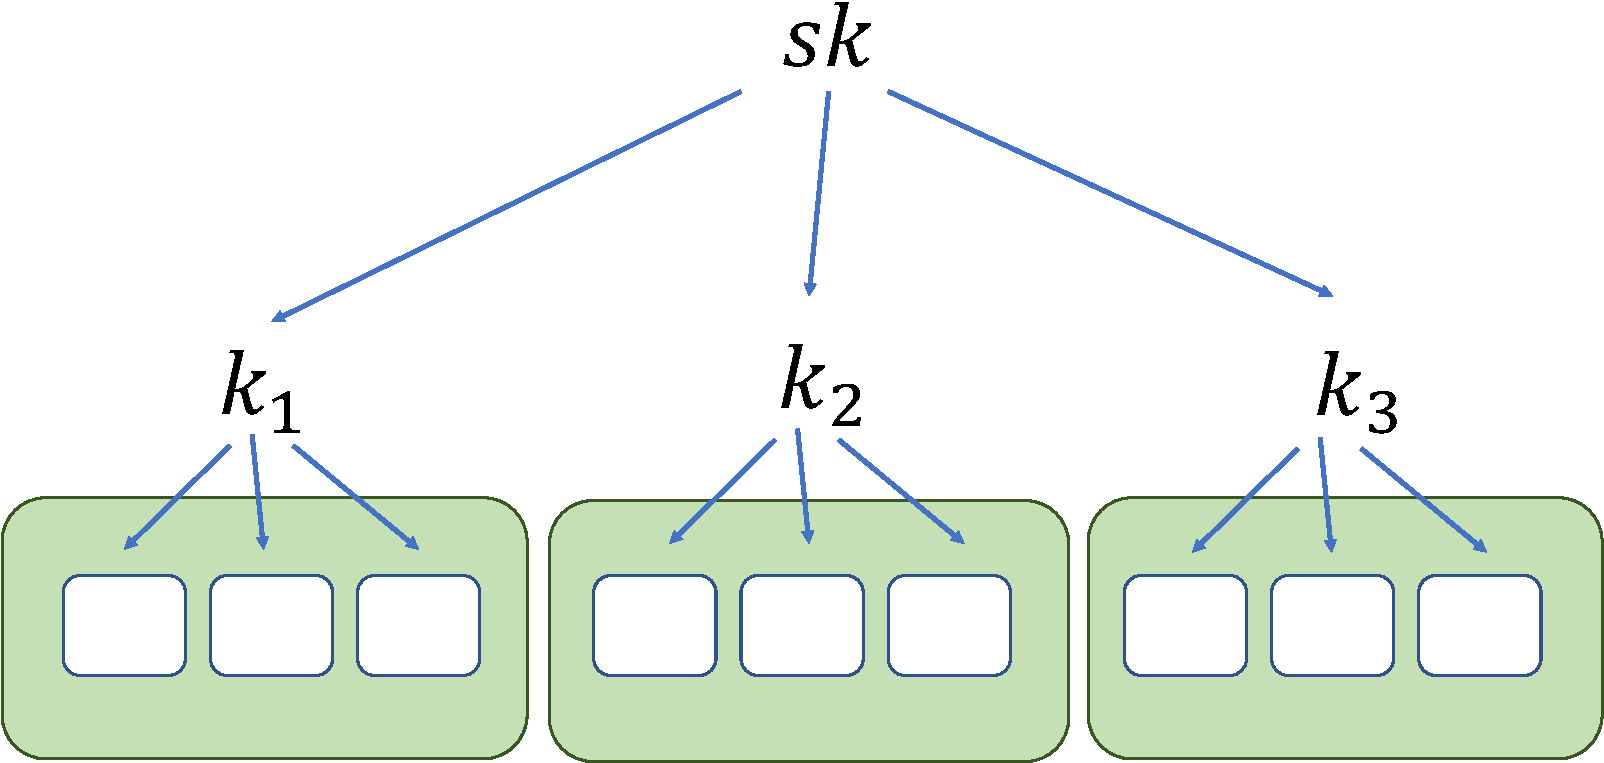
\includegraphics[width=0.5\linewidth]{figs/set-rep.pdf}
    \caption{Two-layer set representation\label{fig:set-rep}. The first layer key expands to $n^{1/4}$ superblock keys. Each superblock key further 
expands to $n^{1/4}$ offsets, one for each chunk in the superblock.}
\end{figure*}

\begin{figure*}[t]
    \centering
    \begin{subfigure}[t]{0.48\textwidth}
        \centering
        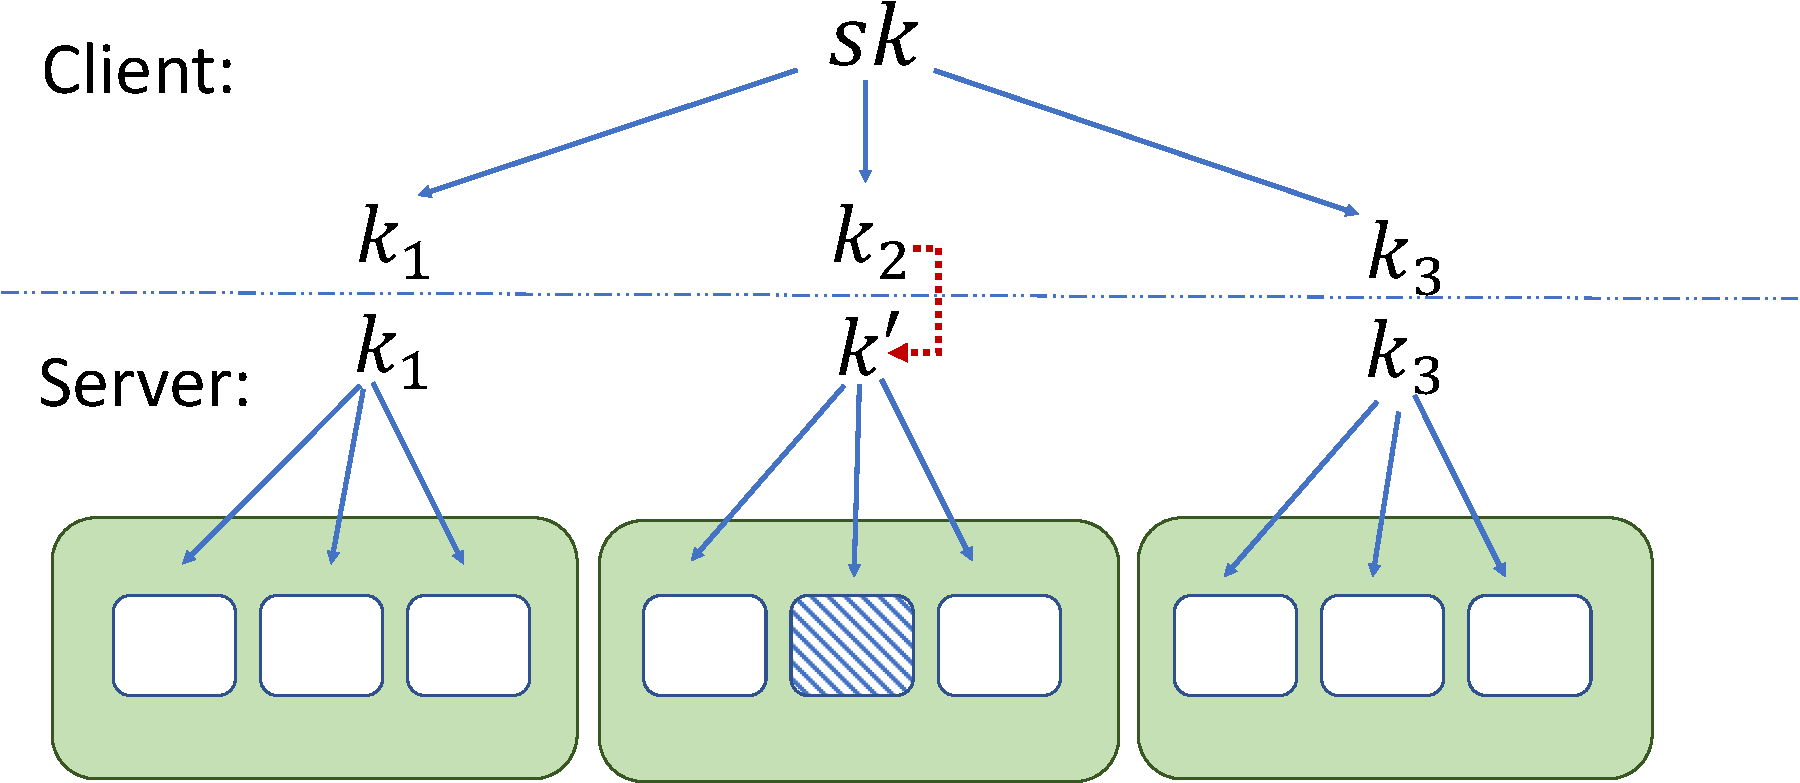
\includegraphics[width=\textwidth]{figs/step1.pdf}
        \caption*{Step 1: The client expands the \ppps key to $n^{1/4}$ superblock 
            keys and replaces the key corresponding to $x$'s superblock with a random key. 
        }\label{fig:step1}
    \end{subfigure}
    \hfill
    \begin{subfigure}[t]{0.48\textwidth}
        \centering
        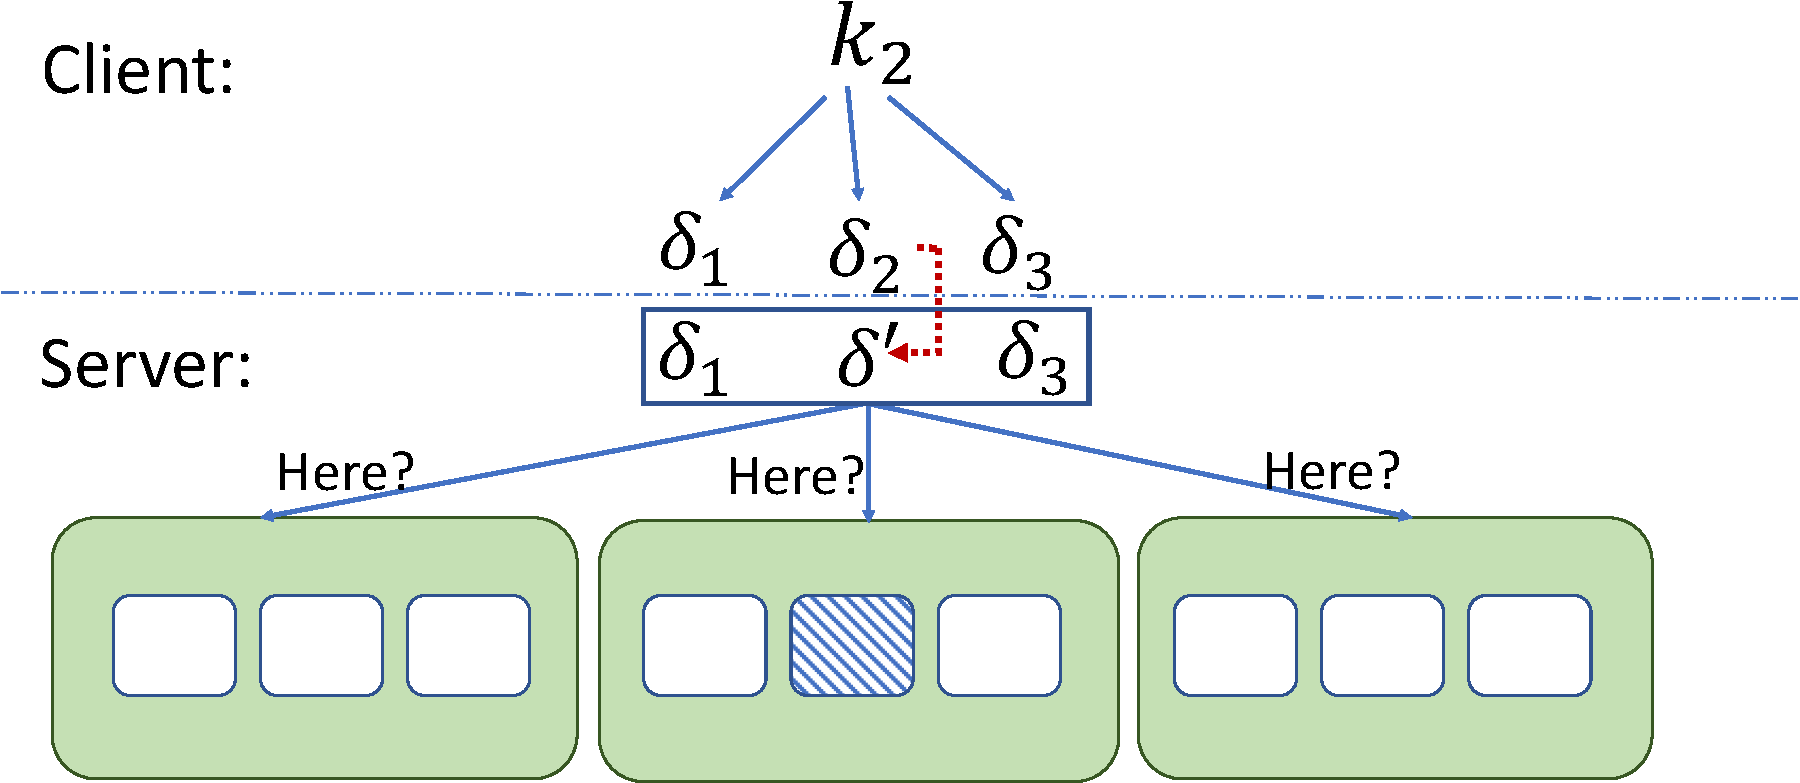
\includegraphics[width=\textwidth]{figs/step2.pdf}
        \caption*{Step 2: The client expands the 
            replaced superblock key to $n^{1/4}$ offsets and replaces $x$'s offset to a random one. 
            The server constructs the candidate sets by plugging these offsets into every superblock. 
        }
        \label{fig:step2}
    \end{subfigure}
    \caption{Illustration about how \ppps is used in our PIR schemes. The client programs the key and the server will decode the list of candidate sets.}
    \label{fig:algo}
\end{figure*}



\paragraph{Size of programmed key and efficiency of ${\sf ListDecode}$.}
Clearly, the programmed key $\sk'$ output by 
${\sf Program}$ has size $O_\lambda(n^{1/4})$.
It is also easy to have a succinct representation of
size $O(\sqrt{n})$ of all $n^{1/4}$ candidate sets output by 
${\sf ListDecode}$.
Specifically, one can first compute the common set $S$ of size $\sqrt{n}$ (we abuse the notation that this set is derived from flattening the matrix $S$ in $\ListDecode$). 
Then, the symmetric difference between the $i$-th candidate set and the common set $S$ is just $2n^{1/4}$ elements (those elements in the $i$-th superblocks). 
So the succinct representation (and hence the efficient algorithm) of $\ListDecode$ takes $O_\lambda(\sqrt{n})$ space and time.


%sets on

%can be recovered from the internal variable $S$ 
%in the ${\sf ListDecode}$ algorithm
%as well as $\{\delta^*_j\}_{j \in \{0, \ldots, %n^{1/4}-1\}}$.
\ignore{
We first write down the common set, $S$, as following:
\[
S=\{\delta_{i,j}+i\cdot n^{3/4} + j\cdot \sqrt{n} \}_{i,j\in \{0,\dots,n^{1/4}-1\}}
\] 
The key is that, the symmetric difference between the $i$-th decoded set $S_i$ and the common set $S$ only has $2n^{1/4}$ elements.
We just remove the elements in the $i$-th superblock and fill that superblock with the offsets of $\delta^*_0,\dots,\delta^*_{n^{1/4}-1}$. Specifically, its full description is:
\[
S_i = \left(S/\{ \delta_{i,j}+ i\cdot n^{3/4} + j\cdot \sqrt{n}\}_{j\in \{0,\dots,n^{1/4}-1\}}\right) \cup \left\{\delta^*_{j}+ i\cdot n^{3/4} + j\cdot \sqrt{n}\right\}_{ j\in \{0,\dots,n^{1/4}-1\}}
\]
This representation only takes $O(n^{1/4})$ extra space and time based on the representation of $S$. 
In total, we have $n^{1/4}$ possible sets.
We simply just store the common set $S$ (which takes $O(\sqrt{n})$ space and time) and store the difference between $S_i$ and $S$ for all $n^{1/4}$ possibilities (where each one takes $O(n^{1/4})$ space and time).
Then, the total time and space cost for $\ListDecode$ is just $O(\sqrt{n})$.
}

\paragraph{Efficient set membership.}
The above construction also supports
$O_\lambda(1)$-time set membership query. 
Given a secret key $\sk$ that has not been programmed, 
to check if some element $x \in {\sf Set}(\sk)$ or not, 
one simply has to check 
\[
\PRF_2(\PRF_1(\sk, \lfloor \ell/n^{1/4}\rfloor), \ \ \ell \text{ mod } n^{1/4}) 
\overset{?}{=} x \text{ mod } n^{1/2}
\text{ where } \ell = %{\sf chunk}(x)
\lfloor x/n^{1/2}\rfloor
\]


\subsection{Proof of Correctness}
To see correctness, 
let $\sk \leftarrow {\sf Gen}(1^\lambda, n)$, 
let $\sk', i^* \leftarrow {\sf Program}(\sk, \chunkid, \delta_\chunkid)$.
Recall that $\sk'$ can be parsed as 
$\sk' = (\{k_i\}_{i\in \{0, \ldots, n^{1/4}-1\}}, 
\{\delta^*_i\}_{i\in \{0, \ldots, n^{1/4}-1\}})$, 
and by construction, we know that 
$i^* = \lfloor \chunkid / n^{1/4}\rfloor$ is the index of the superblock 
that contains 
the chunk $\chunkid$.
Let $j^* := \chunkid \mod n^{1/4}$. 
Let $S_\emptyset := {\sf Set}(\sk)$, 
and we can view $S_{\emptyset}$
as a $n^{1/4} \times n^{1/4}$ matrix.
The correct programmed set $S^*$ is $S_\emptyset$
but replacing the element at index $(i^*, j^*)$
with $\delta_\chunkid$. %+ \chunkid \cdot \sqrt{n}$.

Below, we show that the set $S_i$ output by ${\sf ListDecode}$
is the same as $S^*$.
By %the definition of our algorithms, 
construction, 
in the ${\sf ListDecode}(\sk')$
algorithm, the intermediate set $S$ 
is the same as $S_{\emptyset}$
except for the $i^*$-th row.
Further, the $i^*$-th row of $S_\emptyset$
is the same as 
$\{\delta^*_j\}_{j\in \{0, \ldots, n^{1/4}-1\}}$
but replacing the $j^*$-th element
with $\delta_\chunkid$. %where $j^* := \chunkid \mod n^{1/4}$.
Additionally, the $S_i$ output 
by ${\sf ListDecode}$ is obtained by replacing
the $i^*$-th row of $S$ with 
$\{\delta^*_i\}_{i\in \{0, \ldots, n^{1/4}-1\}}$.




%where 
%$i$ is the superblock containing the $\chunkid$-th 
%chunk.




\subsection{Proof of Security}
We now prove pseudorandomness and private programmability
assuming the security of the underlying $\PRF_1$ and $\PRF_2$.

\paragraph{Pseudorandomness.}
Pseudorandomness follows directly from the pseudorandomness
of the underlying PRFs.

\paragraph{Private programmability.}
We can consider the following sequence of hybrid experiments.
Fix an arbitrary chunk identifier $\chunkid$
and an index $x$ that belongs to the $\chunkid$-th chunk.
Throughout, let $i^* = \lfloor \chunkid/n^{1/4} \rfloor$, let
$j^* = \chunkid \mod n^{1/4}$.

\paragraph{Experiment ${\sf Real}$.}
Recall the definition of the real experiment.
Sample a PRF key $\sk$ such that 
%$x \in {\sf Set}(\sk)$, 
$\PRF_2(\PRF_1(\sk, i^*), j^*) = x \mod \sqrt{n}$.
Let $\delta_\chunkid \getr \{0, 1, \ldots, \sqrt{n}-1\}$,  
and let $\sk', \_ \leftarrow {\sf Program}(\sk, \chunkid, \delta_\chunkid)$, 
output $\sk'$.

\paragraph{Experiment ${\sf Hyb}$.}
%Let $\delta_\chunkid \getr \{0, 1, \ldots, \sqrt{n}-1\}$.
Same as ${\sf Real}$ except with the following modification: 
when executing the ${\sf Program}(\sk, \chunkid, \delta_\chunkid)$ 
algorithm
instead of using the $k_0, \ldots, k_{n^{1/4}-1}$
keys that are expanded using $\PRF_1(\sk, \cdot)$, 
sample 
$k_0, \ldots, k_{n^{1/4}-1}$
at random subject to 
$\PRF_2(k_{i^*}, j^*) = x \mod \sqrt{n}$.

\begin{lemma}
Suppose that $\PRF_1$ is secure. 
Then, ${\sf Hyb}$ 
is computationally indistinguishable from ${\sf Real}$.
\label{lem:privateprog1}
\end{lemma}
\begin{proof}
%\elaine{FILL}
Suppose there is an efficient adversary $\mcal{A}$ that can distinguish
${\sf Real}$ and ${\sf Hyb}$ with non-negligible probability. 
We can construct the following efficient reduction 
$\mcal{B}$
which can distinguish a PRF from a random function 
with non-negligible probability. 
Basically, $\mcal{B}$ 
is interacting with its own challenger
who either answers queries using a PRF or using a truly random function.
$\mcal{B}$
will query its own challenger on the inputs 
$0, 1, \ldots, n^{1/4}-1$, 
and it will obtain 
$k_0, \ldots, k_{n^{1/4} - 1}$ from 
its challenger.
It will check if $k_{i^*}$
satisfies the relation 
$\PRF(k_{i^*}, j^*) = x \mod \sqrt{n}$. 
If not, $\mcal{B}$ aborts and outputs $0$. 
Otherwise, it runs the ${\sf Program}$ algorithm where it plugs in 
the terms $k_0, \ldots, k_{n^{1/4} - 1}$  
as the superblock keys.
It gives the resulting $\sk'$
to $\mcal{A}$. 
%Since the relationship 
%$\PRF(k_{i^*}, j^*) = x \mod \sqrt{n}$
Henceforth, we use $b = 0$ to denote the world  
in which $\mcal{B}$'s  challenger 
uses 
a truly random function, and we use $b = 1$ to denote
the world in which $\mcal{B}$'s challenger uses a randomly sampled PRF function.
We use the notation $\Pr_b[\cdot]$
to denote the probability of events in world $b \in \{0, 1\}$. 
Let $G$ be the good event that 
the relation 
$\PRF(k_{i^*}, j^*) = x \mod \sqrt{n}$
is satisfied.

\[
\Pr_b[\mcal{B} \text{ outputs } 1]
= 
0 \cdot \Pr_b [\overline{G}]
+ \Pr_b[ \mcal{A} \text{ outputs } 1 | G] \cdot \Pr_b[G]
\]

We know that $\Pr_0[G] = 1/\sqrt{n}$ which is non-negligible.
If the PRF is secure, then 
it must be that $|\Pr_1[G] - \Pr_0[G]| \leq \negl(\lambda)$
due to a straightforward reduction to PRF security.
Therefore, we have that 
\begin{align*}
 & \left|\Pr_1[\mcal{B} \text{ outputs } 1]
- \Pr_0[\mcal{B} \text{ outputs } 1]\right|\\
 = & 
\left| \Pr_1[ \mcal{A} \text{ outputs } 1 | G] \cdot \Pr_1[G]
- 
\Pr_0[ \mcal{A} \text{ outputs } 1 | G] \cdot \Pr_0[G]
\right|\\
\geq & 
\left|\Pr_1[ \mcal{A} \text{ outputs } 1 | G] 
- 
\Pr_0[ \mcal{A} \text{ outputs } 1 | G] \right|\cdot \frac{1}{\sqrt{n}}
- \negl(\lambda)
\end{align*}

Observe also that in world $0$, conditioned on $G$,
$\mcal{A}$'s view in the experiment is identically distributed
as ${\sf Hyb}$.  
In world $1$, conditioned on $G$,
$\mcal{A}$'s view in the experiment is identically distributed
as ${\sf Real}$.  
Therefore, the term 
\[\left|\Pr_1[ \mcal{A} \text{ outputs } 1 | G]
-
\Pr_0[ \mcal{A} \text{ outputs } 1 | G] \right|\]
represents $\mcal{A}$'s advantage
in distinguishing ${\sf Real}$ and ${\sf Hyb}$.
We can now conclude that if $\mcal{A}$ can distinguish
${\sf Real}$ and ${\sf Hyb}$ with non-negligible probability,
then $\mcal{B}$ can break PRF security with non-negligible probability.
\end{proof}


\paragraph{Experiment ${\sf Ideal}$.}
The ${\sf Ideal}$ experiment 
is almost the same as ${\sf Hyb}$ except with the following modification: 
when outputting the $\sk'$, 
instead of using the $\delta_0, 
\ldots, \delta_{j^*-1},  
\delta_{j^*+1},  
\delta_{n^{1/4}-1}$
terms derived from evaluating $\PRF_2(k_{i^*}, \cdot)$ 
at the points $0, 1, \ldots, j^*-1, j^*+1, \ldots, n^{1/4} -1$, 
we now sample $\delta_0,  
\ldots, \delta_{j^*-1},  
\delta_{j^*+1},  
\delta_{n^{1/4}-1}$
at random from $\{0, \ldots, n^{1/2}-1\}$ instead.

Observe that in the 
${\sf Ideal}$
experiment, we no longer make use of knowledge of the query $x$.
Therefore, %we can view the output 
the description of the ${\sf Ideal}$ 
experiment also uniquely specifies the simulator ${\sf Sim}$
we want to construct.

\begin{lemma}
Suppose that $\PRF_2$
is secure. Then, ${\sf Ideal}$ is computationally
indistinguishable from ${\sf Hyb}$.
\label{lem:privateprog2}
\end{lemma}
\begin{proof}
It suffices to show that the following to probability ensembles are
computationally indistinguishable
for any fixed $\delta^* \in \{0, 1, \ldots, \sqrt{n}-1\}$,
and $j^* \in \{0, 1, \ldots, n^{1/4} -1\}$.
\begin{enumerate}[leftmargin=5mm]
\item 
${\sf Distr_0}$:
Output a randomly sampled vector 
$\delta_0, \ldots, \delta_{n^{1/4}-1} 
\in \{0, 1, \ldots, \sqrt{n}-1\}^{n^{1/4}}$.
\item  
${\sf Distr_1}$:
Sample a PRF key $k$ subject to 
$\PRF_2(k, j^*) = \delta^*$.  
Sample $\delta' \in \{0, 1, \ldots, \sqrt{n}-1\}$ at random. 
For $j \in \{0, 1, \ldots, n^{1/4}-1\}$, 
compute $\delta_j = \PRF_2(k, j)$.
Output 
$\delta_0, \ldots, \delta_{j^*-1}, \delta', 
\delta_{j^*+1}, \ldots, \delta_{n^{1/4}-1}$.
\end{enumerate}

If there is an efficient adversary $\mcal{A}$ that can distinguish
between the above 
${\sf Distr}_0$ 
and  
${\sf Distr}_1$ 
with non-negligible probability, we can construct an efficient 
reduction $\mcal{B}$
that can distinguish
whether it is interacting with a random oracle 
or a randomly chosen PRF function.
Basically, $\mcal{B}$ 
sends the inputs $0, \ldots, n^{1/4}-1$ to the oracle 
it is interacting with, and gets back
$\delta_0, \ldots, \delta_{n^{1/4}-1}$.
If $\delta_{j^*} \neq \delta^*$, 
then $\mcal{B}$ aborts and outputs $0$. 
Otherwise, it 
replaces $\delta_{j^*}$ with a random value
from $\{0, \ldots, n^{1/2}-1\}$
and gives the resulting vector to $\mcal{A}$.
Suppose $\mcal{B}$ is interacting with a random oracle,
then conditioned on the good event 
$\delta_{j^*} = \delta^*$, $\mcal{A}$'s view
is identically distributed as ${\sf Distr}_0$.
On the other hand, suppose $\mcal{B}$ is interacting with a PRF,
then conditioned on the good event 
$\delta_{j^*} = \delta^*$, $\mcal{A}$'s view
is identically distributed as ${\sf Distr}_1$.
The rest of the proof can be completed due
to a similar probability calculation as 
\Cref{lem:privateprog1}.
\end{proof}





